\documentclass[11pt]{article}
\usepackage[margin=1in]{geometry}
\usepackage{amsmath,amsthm,amssymb}
\usepackage{enumitem, graphicx, float, caption}
\usepackage{amsmath}
\usepackage{bm}
\usepackage{parskip}
\usepackage{lipsum}
\usepackage{tikz}
\usepackage{listings}
\usepackage{xcolor}
\usepackage{float}
\usepackage{subcaption}
\usepackage{graphicx}
\usepackage{xfrac}
\usepackage[utf8]{inputenc}
\usetikzlibrary{arrows.meta}

\definecolor{codegreen}{rgb}{0,0.6,0}
\definecolor{codegray}{rgb}{0.5,0.5,0.5}
\definecolor{codepurple}{rgb}{0.58,0,0.82}
\definecolor{backcolour}{rgb}{0.95,0.95,0.92}

\lstdefinestyle{mystyle}{
    backgroundcolor=\color{backcolour},
    commentstyle=\color{codegreen},
    keywordstyle=\color{magenta},
    numberstyle=\tiny\color{codegray},
    stringstyle=\color{codepurple},
    basicstyle=\ttfamily\tiny,
    breakatwhitespace=false,
    breaklines=true,
    captionpos=b,
    keepspaces=true,
    numbers=left,
    numbersep=5pt,
    showspaces=false,
    showstringspaces=false,
    showtabs=false,
    tabsize=2
}

\lstset{xleftmargin=.020\textwidth, xrightmargin=.020\textwidth}

\setcounter{MaxMatrixCols}{26}
\setlength\parindent{0pt}
\counterwithin{equation}{enumi}


\begin{document}
    \noindent Nathan Burwig \\
    Math 87 HW 5 \\
    Due 10/19/2022
    
    \hrulefill

    \textbf{Strolling Down an Infinite Street}

        Suppose you’re standing on a street with buildings labelled by 
        the integers (specifically, you’re in front of the building labelled 
        0, and suppose that the indices are increasing to the right). 
        Suppose that every minute you flip a coin. If the coin is heads 
        you walk right and if the coin is tails you walk left.
    
    \begin{enumerate}
        \item \textbf{Explain why your position (i.e. the building you’re in front of) 
            as a function of time can be modeled as a Markov Chain}

            We know your position in this system is determined
            probabilistically. Ie, moving from one node to the node to the left has a 1/2
            chance of happening, so our chance of being at a particular node at
            any time t is given by the probability of getting to the nodes we
            were previously on. We could make this into a stochastic matrix,
            but given that we are dealing with an integer line, that would make
            it an infinite matrix. In anycase, the values would be largely zero
            apart from adjacent nodes in which case the probabilities in the
            matrix would be 1/2.

            Since our system can be represented as a stochastic matrix, and we
            can draw out a finite state machine for this system, we know that
            it is in fact a Markov chain.

            I've also assumed that infinite markov chains are allowed, but I
            don't actually believe they are. At least, there doesn't seem to be
            any particular meaning to having an infinite Markov chain vs a very
            large chain. For all intents and purposes, I will assume out street
            ends at some point very far away from the start, such that I can
            avoid any infinity problems. I know the problem says infinite
            street I just also know that things get wonky at infinity, so in
            classic physicist fashion I will approximate infinity as large N :).
            \medskip

        \item \textbf{Is the distance from where you started as a function of time a
            Markov Chain?}

            The distance from where we started, unlike the initial problem, is
            \textit{not} an integer line, but instead a natural number line, as
            distance cannot be negative. Thus we have an FSM where we start at
            zero. After flipping a coin, we have a 100\% chance of being at
            distance 1, and from then on, whatever node you are at, you have a
            50\% chance of moving either closer to or farther from zero. So you
            can still describe your next state, at time t + 1, as a probability
            from your current state, which means that this system is also a
            Markov chain.
            \medskip

        \item \textbf{Now suppose that every minute you flip two coins. If both are 
            heads, you move right, if both are tails you move left and 
            otherwise you stay put. Is your distance from where you 
            started a Markov chain in this scenario? How do you expect this 
            to compare to the process described in part 2?}

            Your distance from zero would still be a Markov chain for the
            same reason as above. The only real difference is that you have
            self-cycles at each node where you can loop back onto the node you
            are on with a 1/2 probability. At node zero, you have a 50\% chance
            of moving to distance 1, and from there, a 1/4 chance of moving
            either left or right, and 1/2 of staying put. Thus you can model
            this as a Markov chain.
            \medskip

        \item For the single coin experiment, we know that at time zero we sit
            at node zero with 100\% probability, thus there is a zero percent
            chance of being on an odd node. At t = 1, we are either on -1 or 1
            with 100\% probability, thus we are on odd with 100\%. This pattern
            will continue, and if our time step is odd (ie $t\;\%\;2 \neq 0$),
            then we are on odd with 100\%, and otherwise we are on odd with
            0\%.

            The case of two coins is slightly more complex, but not terribly.
            We know that when we flip coins the first time, it is a 50 50
            chance that we move at all. If we do move, we are on a an odd,
            which means at time step one, we are on an odd with 50\%. At each
            time step following, we have a 50 50 chance of moving, which means
            that we will either remain on the odd we are on, or we will move
            onto an even, or vice versa. Thus at \textbf{every} timestep
            \textit{apart from time t = 0} we have a 50\% chance of being on an
            odd.

            Just for fun, I went ahead and simulated 100 million people walking
            in this way, and was able to confirm that the probabilities above
            are in fact accurate.
    \end{enumerate}
    \medskip

    \textbf{Rain or Shine}
    
    On Planet X, the weather is strangely predictable: The weather is always 
    either sunny, rainy, foggy or snowy. If it rains today, its sunny tomorrow. 
    If it is sunny today, its rainy tomorrow. If its foggy today, its not sunny 
    tomorrow. Finally, the weather is never the same two days in a row. 
    Apart from these rules, the weather is completely random, in that if 
    e.g. its foggy today it is equally likely to be either rainy or snowy 
    tomorrow. You live on Planet X and are trying to figure out what to wear 
    this week, so you’d like to develop a model for the weather.

    \begin{enumerate}
        \item \textbf{Explain why the weather can be modeled as a Markov chain. 
            Write out the transition matrix, and draw the corresponding 
            finite state machine}

            We can model the weather as a markov chain because we know the
            probabilities of going from a given state to another state. Our
            next state is probabilistically determined from our current state,
            and all the sates are possible to arrive at (depending on where you
            start I suppose). It has the following transition matrix.
            \[
                S = 
                \begin{bmatrix}
                    0   &   1   &   \sfrac{1}{2} &   \sfrac{1}{3} \\
                    1   &   0   &   0            &   \sfrac{1}{3} \\
                    0   &   0   &   0            &   \sfrac{1}{3} \\
                    0   &   0   &   \sfrac{1}{2} &   0            \\
                \end{bmatrix}
            \]
            Which we arrive at based on the following finite state machine...

            \begin{center}
                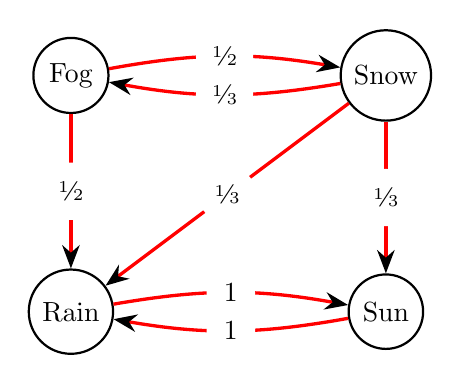
\begin{tikzpicture}
                    \begin{scope}[every node/.style = {circle, thick, draw}]
                        \node (R) at (0, 1)    {Rain};
                        \node (S) at (4, 1)    {Sun};
                        \node (W) at (4, 4)    {Snow};
                        \node (F) at (0, 4)    {Fog};
                    \end{scope}

                    \begin{scope}[>={Stealth[black]},
                            every node/.style={fill=white,circle},
                            every edge/.style={draw=red,very thick}]

                        \path [->] (R) edge[bend left=10] node {1} (S);
                        \path [->] (S) edge[bend left=10] node {1} (R);

                        \path [->] (F) edge node {\sfrac{1}{2}} (R);
                        \path [->] (F) edge[bend left=10] node {\sfrac{1}{2}} (W);

                        \path [->] (W) edge node {\sfrac{1}{3}} (S);
                        \path [->] (W) edge node {\sfrac{1}{3}} (R);
                        \path [->] (W) edge[bend left=10] node {\sfrac{1}{3}} (F);
                    \end{scope}
                \end{tikzpicture}
            \end{center}

        \item \textbf{Check whether the conditions for the Perron-Frobenius 
            theorem is satisfied for this problem (aperiodic and strongly 
            connected). Explain your reasoning.}

            We know that the Perron-Frobenius theorem is satisfied if the
            transition diagram for a Markov Chain is strongly connected and
            aperiodic. We can note, that if we are at a rainy day, or a sunny
            day, there is no possible way we can arrive at a snowy or foggy
            day, thus the graph is not strongly connected as there is not a
            sequence of edges that can take us from Rainy to Foggy. Thus, the
            Perron-Frobenius theorem is not satisfied for this Markov Chain.

        \item \textbf{Do you expect power iteration to be effective for 
            computing the greatest eigenvector of your transition matrix?}

            I do not expect power iteration to be an effective method for
            computing the greatest eigenvector of the transition matrix. If we
            use power iteration, at some point the terms that are less than 1
            will go to zero, and we will be left with two terms that are just
            1, which will not help us determine the greatest eigenvector as
            there will be two with the same value.

        \item \textbf{Find the eigenvalue decomposition for the transition matrix, 
            and the associated eigenvectors. Explain why these values confirm 
            your answer to part 2.}

            We can find the eigenvalue decomposition of our stochastic matrix
            by using wolfram! Because I find it easier than doing it using
            python. We find the following values for our eigenvalues...
            \[
                \lambda_1 = -1\;\;\; 
                \lambda_2 = 1\;\;\;
                \lambda_3 = -\frac{1}{\sqrt{6}} \;\;\; 
                \lambda_4 = \frac{1}{\sqrt{6}} 
            \]
            With corresponding eigenvectors...
            \[
                v_1 = \begin{bmatrix} -1 & 1 & 0 & 0 \end{bmatrix},\;\;
                v_2 = \begin{bmatrix}  1 & 1 & 0 & 0 \end{bmatrix} 
            \]
            \[
                v_3 = \begin{bmatrix} -.4367 & .2532  & -.8165 & 1 \end{bmatrix},\;\;
                v_4 = \begin{bmatrix} -.7640 & -1.053 & 0.8165 & 1 \end{bmatrix}
            \]

            We can immediately see that the eigenvalues of this transition
            matrix show our response to part 2 was, in fact, correct. We know
            that Perron-Frobenius dictates that a Markov chain satisfying the
            theorem's conditions will only have one eigenvalue with value
            $|\lambda| = 1$ and all other eigenvalues whose absolute values are
            less than one. This clearly isn't true for the case of $\lambda_1$
            and $\lambda_2$.

        \item \textbf{Suppose that the “weather rules” change so that if its 
            sunny today, it is equally likely to be snowy or rainy tomorrow. 
            Write out the new transition matrix, associated finite state 
            machine, and determine whether the conditions for the Perron-
            Frobenius are satisfied. Compute the eigenvalue decomposition
            and compare to the previous set of eigenvalues.}

            We can remodel our state machine to reflect the change in the
            rules. It will look as follows...

            \begin{center}
                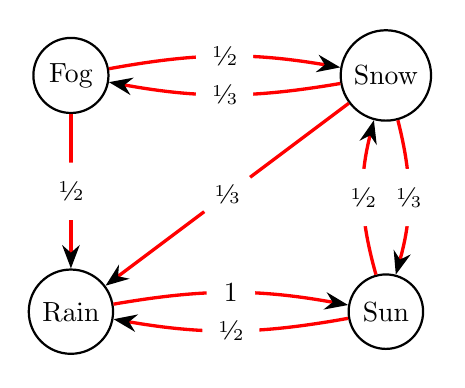
\begin{tikzpicture}
                    \begin{scope}[every node/.style = {circle, thick, draw}]
                        \node (R) at (0, 1)    {Rain};
                        \node (S) at (4, 1)    {Sun};
                        \node (W) at (4, 4)    {Snow};
                        \node (F) at (0, 4)    {Fog};
                    \end{scope}

                    \begin{scope}[>={Stealth[black]},
                            every node/.style={fill=white,circle},
                            every edge/.style={draw=red,very thick}]

                        \path [->] (R) edge[bend left=10] node {1} (S);
                        \path [->] (S) edge[bend left=10] node {\sfrac{1}{2}} (R);
                        \path [->] (S) edge[bend left=15] node {\sfrac{1}{2}} (W);

                        \path [->] (F) edge node {\sfrac{1}{2}} (R);
                        \path [->] (F) edge[bend left=10] node {\sfrac{1}{2}} (W);

                        \path [->] (W) edge[bend left=15] node {\sfrac{1}{3}} (S);
                        \path [->] (W) edge node {\sfrac{1}{3}} (R);
                        \path [->] (W) edge[bend left=10] node {\sfrac{1}{3}} (F);
                    \end{scope}
                \end{tikzpicture}
            \end{center}

            And our transition matrix will also reflect these changes in the
            following ways...
            \[
                S' = 
                \begin{bmatrix}
                    0   &   \sfrac{1}{2}    &   \sfrac{1}{2} &   \sfrac{1}{3} \\
                    1   &   0               &   0            &   \sfrac{1}{3} \\
                    0   &   0               &   0            &   \sfrac{1}{3} \\
                    0   &   \sfrac{1}{2}    &   \sfrac{1}{2} &   0            \\
                \end{bmatrix}
            \]
            Now we ask if the Perron-Frobenius theorem is satisfied. We can see
            know that the graph is strongly connected, as you can devise a path
            from one node to any other node.

            We do have to determine whether or not this graph is aperiodic. We
            can see that it must be, as no integer greater than 1 can divide
            the longest cycle on the graph, so certainly no integer greater
            than one can divide any smaller length paths. The longest path on
            this graph does not exceed four, and is only ever a fraction,
            and never a whole integer greater than 1. Thus no integer greater
            than one could divide it, and it is aperiodic and strongly
            connected, satisfying Perron-Frobenius. 

            We now expect to see only one eigenvalue with value 1 and the 
            rest all being less than one. Let us see.
            \[
                \lambda_1' = 1\;\;\; 
                \lambda_2' \approx -.789 \;\;\;
                \lambda_3' \approx -.211 \;\;\; 
                \lambda_4' = 0
            \]
            So we can see that the eigenvalues for this new problem, are a bit
            different from the original and, as expected, the largest value of
            the eigenvalues is $\lambda_1'$ which is exactly 1, all the rest
            having abosolute values less than 1. So we can see here how
            Perron-Frobenius plays out.

    \end{enumerate}

\end{document}
